% !TeX program = lualatex
\documentclass[9pt,aspectratio=169]{beamer}
\graphicspath{{figuras/}{./}}
\usepackage[spanish]{babel}
%\usepackage[utf8]{inputenc} % Solo desbloquear con pdfLaTeX
\usepackage{tikz}
\usepackage{booktabs}
\usepackage{csquotes}
\usepackage[backend=biber,style=ieee]{biblatex}
    \addbibresource{biblio.bib}
    \renewcommand*{\bibfont}{\scriptsize} % Cambiar el tamaño de la bibliografía.
    \AtEveryBibitem{\clearfield{title}}
\usepackage{xcolor}
\usepackage{caption}
\usepackage{multicol}
\usepackage{dirtytalk}
\usepackage[shortlabels]{enumitem}
\usepackage[version=4]{mhchem}
\usepackage{colortbl}

%%% TEMAS Y COLORES %%%
%%% FUENTE
% Si la fuente no carga, revisar: https://www.overleaf.com/learn/latex/Questions/I_have_a_custom_font_I%27d_like_to_load_to_my_document._How_can_I_do_this%3F#Using_custom_fonts_with_XeLaTeX_and_LuaLaTeX para agregar una fuente personalizada al proyecto.
\usepackage{fontspec}
\usepackage{fontawesome}
%\setsansfont{Arial} % Sans. Titles. Good options include: {Inter, Roboto, Cabin, Arial}

%%% TEMA
\usetheme{Boadilla}

%%% COLORES
\definecolor{ITESOblue}{HTML}{10427a}
\definecolor{PAPgreen}{HTML}{86c400}
\definecolor{PAPlightblue}{HTML}{009fe3}
\definecolor{PAPorange}{HTML}{ff671c}

\setbeamercolor{structure}{fg=ITESOblue}
\setbeamercolor{frametitle}{bg=ITESOblue,fg=white}

%%% CONFIGURACION DE BEAMER %%%
\usefonttheme{structurebold} % Títulos en negritas.
\useinnertheme{circles} % Viñetas como círculos.
\setbeamertemplate{caption}[numbered] % Número en las captions.
\captionsetup{font=scriptsize, justification=centering} % Tamaño de las captions.

%% Adornos de portada
\titlegraphic{
\begin{tikzpicture}[overlay,remember picture]
    \node[anchor=south, yshift=-3pt] at (current page.south){
        \includegraphics[width=1.05\textwidth]{adorno_maintitle.pdf}
    };
\end{tikzpicture}
}

%% Diapositivas de título para secciones
\AtBeginSection[]{
  \begin{frame}
  \vfill
  \centering
  \begin{beamercolorbox}[sep=8pt,center,shadow=true,rounded=true]{title}
    \usebeamerfont{title}\insertsectionhead\par%
  \end{beamercolorbox}
  \vfill
  \end{frame}
}
%\AtBeginSection[]{
%    \begin{frame}{Contenidos}
%        \begin{multicols}{2}
%            \tableofcontents[currentsection,hideothersubsections]
%        \end{multicols}
%        \begin{tikzpicture}[overlay,remember picture]
%            \node[anchor=south, yshift=-5.25pt] at (current page.south){
%                \includegraphics[width=1.05\textwidth]{adorno-tabladecontenidos.pdf}
%            };
%        \end{tikzpicture}
%    \end{frame}
%}

%% Usar fontawesome como viñetas
\newcommand{\usageitem}[1]{
  \item[ {\makebox[2em]{\strut #1}} ]
}
\newcommand{\objetivo}{ \usageitem{\centering\color{ITESOblue}\faBullseye} }
\newcommand{\conclusion}{ \usageitem{\centering\color{ITESOblue}\faArrowCircleRight} }
\newcommand{\plus}{ \usageitem{\centering\color{ITESOblue}\faPlusCircle} }

%%% INFORMACION DE LA PRESENTACION %%%
\title[GWAS maíz Ancho]{\large Estudio de Asociación de Genoma Completo (GWAS) en maíz Ancho (\textit{Zea mays} L.) nativo para la identificación de genes relacionados a la respuesta hidrotrópica}

\subtitle{En colaboración con: IBt --- UNAM} % Presentation subtitle, remove this command if a subtitle isn't required

\author[IBT. Olvera-Hernández]{\textit{Ing. en Biotecnología}, Roberto Olvera Hernández \\ {\footnotesize \textbf{Directora PAP:} Dra. Glayds I. Cassab López}} % Presenter name(s), the optional parameter can contain a shortened version to appear on the bottom of every slide, while the main parameter will appear on the title slide

\institute[ITESO]{\normalsize \textcolor{ITESOblue}{Instituto Tecnológico y de Estudios Superiores de Occidente,} \\ Departamento de Procesos Tecnológicos e Industriales} % Your institution, the optional parameter can be used for the institution shorthand and will appear on the bottom of every slide after author names, while the required parameter is used on the title slide and can include your email address or additional information on separate lines

\date[\today]{{\scriptsize Proyecto de Aplicación Profesional (PAP) 4G03} \\ {\small Programa de Apoyo a Centros de Investigación Externos II} \\ {\footnotesize \today}} % Presentation date or conference/meeting name, the optional parameter can contain a shortened version to appear on the bottom of every slide, while the required parameter value is output to the title slide

% -----------------------
%%% INICIAR DOCUMENTO %%%
% -----------------------
\begin{document}
\nocite{*}
{
    \setbeamertemplate{headline}{}
    %%% PORTADA %%%
    \begin{frame}
        \vspace{20pt}
        \maketitle
    \end{frame}
}
\addtocounter{framenumber}{-1}

%%% TABLA DE CONTENIDOS %%%
\begin{frame}
    \frametitle{Contenidos}
        \tableofcontents
\end{frame}

%%% Introducción
\section{Introducción}
%%%% Importancia cultural
\begin{frame}
    \frametitle{Problemática}
    \framesubtitle{El maíz Ancho es sustento de vida}

    \begin{center}
        \includegraphics[width=0.95\textwidth]{maiz-ancho-importanci.png}
    \end{center}
\end{frame}

\subsection{Problemática}
\begin{frame}
    \frametitle{Problemática}
    \framesubtitle{}

    \begin{center}
        \includegraphics[width=0.95\textwidth]{arbol-problemas.pdf}
    \end{center}
\end{frame}

%%%% Alternativa Propuesta
\subsection{Alternativa Propuesta}
\begin{frame}
\frametitle{Alternativa Propuesta}
\framesubtitle{Mejoramiento Evolutivo-Participativo}

\begin{columns}[c]
% Lista de definiciones sobre Mejoramiento Participativo
\begin{column}{0.45\textwidth}
    \textbf{Fundamentos del \say{Mejoramiento Evolutivo-Partitipativo}:}\\
    Establecer una sinergia \textit{agricultor-investigador}\\
    \begin{itemize}
        \item Características deseadas \textit{por} campesinos.
        \item Crear nuevas variedades a partir poblaciones locales.
        \item Aplicación a nivel global desde 1996 \cite{witcombe-1996-mejoramiento-a,witcombe-1996-mejoramiento-b} .
    \end{itemize} 

    \vspace{1em}

    \begin{exampleblock}{¿Qué característica nos interesa?}
        Mejorar la \textbf{respuesta hidrotrópica (RH)} de las raíces en \textit{Zea mays} L. puede ayudar a combatir la sequía.
    \end{exampleblock}
\end{column}

% Imágenes
\begin{column}{0.45\textwidth}
    \begin{figure}[htb]
        \centering
        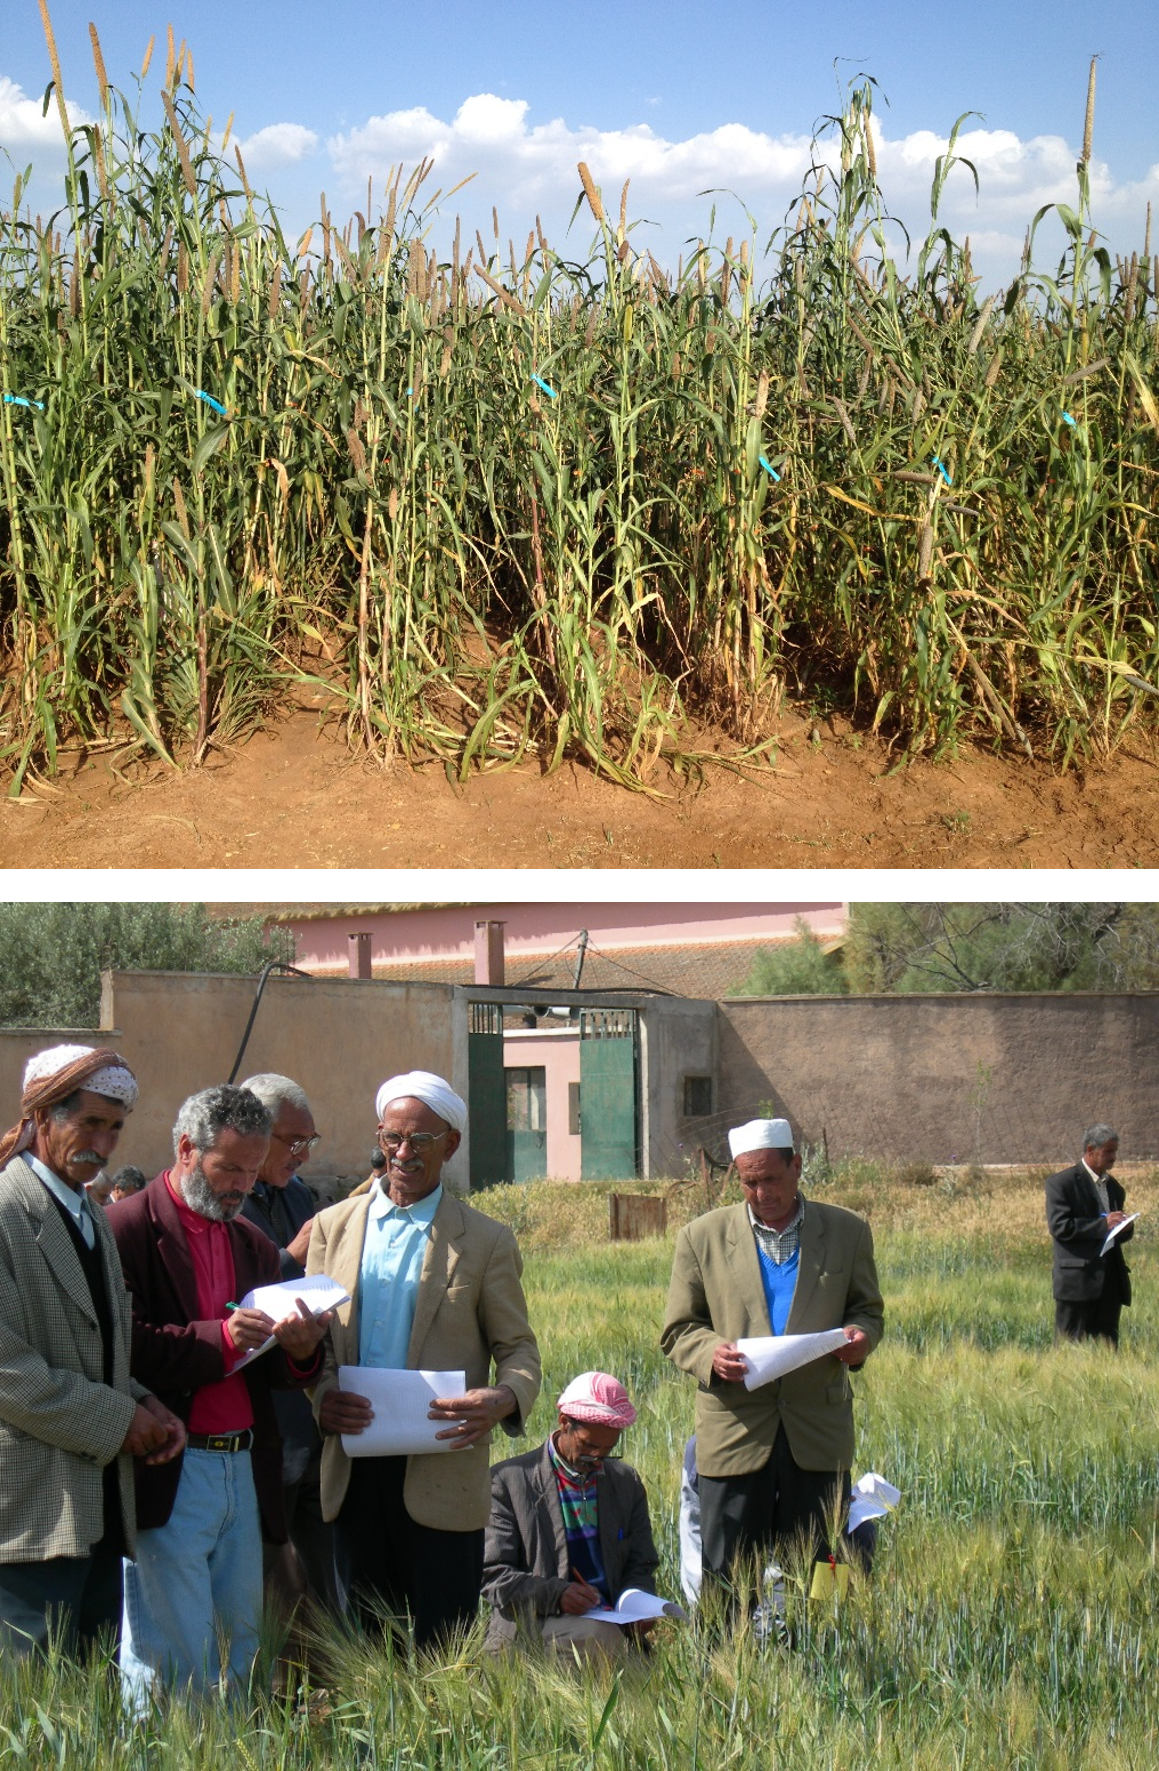
\includegraphics[height=2.35in]{mejoramiento-participativo.png}
        \caption{El mejoramiento participativo es un marco de trabajo científico que toma en cuenta su comunidad.}
        \label{fig:mejoramiento-participativo}
    \end{figure}
\end{column}
\end{columns}
    
\end{frame}

%%%% Respuesta Hidrotrópica
\begin{frame}
  \frametitle{Alternativa Propuesta}
  \framesubtitle{Respuesta Hidrotrópica}

  \begin{columns}[c]

    % Imágenes de hidrotropismo
    \begin{column}{0.45\textwidth}
      \begin{figure}[htb]
        \centering
        \includegraphics[width=\textwidth]{root-hydrotropism.png}
        \caption{Diagrama representativo de los mecanismos de RH en plántulas de \textit{A. thaliana}. Las raíces tienen una preferencia hacia la percepción de gradientes de humedad, en vez de la gravedad. Recuperado de \textcite{eapen-2005-hidrotropismo}.}
        \label{fig:root-hydrotropism}
      \end{figure}
    \end{column}

    % Qué es el hidrotropismo
    \begin{column}{0.45\textwidth}
      {\small\color{darkgray}
      \textbf{Tropismos:} Mecanismos de las plantas para crecer diferencialmente sus órganos a partir de estímulos.
      }\medskip

      \textbf{Hidrotropismo/Respuesta hidrotrópica:} Tropismos \textbf{\color{PAPgreen} radiculares} para encontrar \textbf{\color{PAPlightblue} agua}. 

      \begin{itemize}
        \item Tropismo relativamente nuevo, redescubierto en 1985 por \textcite{jaffe-1985-hidrotropismo}. 
        \item Poca información sobre sus mecanismos moleculares.
        \item Investigaciones en \textit{A. thaliana} mostraron posibles genes \textit{MIZ1} \cite{kobayashi-2007-miz1} y \textit{MIZ2} \cite{miyazawa-2009-miz2}.
      \end{itemize}
      
    \end{column}
  \end{columns}

\end{frame}

%%%% Objetivos
\subsection{Objetivos}
\begin{frame}
    \frametitle{Objetivos}

    %%% GENERAL %%%
    \begin{block}{\bfseries\faBullseye\hspace{0.5em}\LARGE Generales}
        {\Large Encontrar marcadores moleculares relacionados a la respuesta hidrotrópica (RH) en maíz Ancho (\textit{Zea mays} L.) de cultivos nativos en Morelos.}
    \end{block}

    \bigskip

    %%% ESPECIFICOS %%%
    {\LARGE\bfseries\color{ITESOblue} Específicos}\\ \medskip 
    {\large
        \setlist[enumerate,1]{leftmargin=12mm}
        \begin{multicols}{2}
            \begin{enumerate}[itemsep=6pt,topsep=6pt]
                \objetivo Análisis primario y limpieza de \textit{dataset} de secuenciación.
                \objetivo Análisis estadístico de datos fenotípicos.
                \objetivo Control de calidad de datos genotípicos.
                \objetivo Realizar GWAS.
                \objetivo Identificar SNPs y genes asociados a RH.
                \objetivo Encontrar función biológica de genes.
            \end{enumerate}
        \end{multicols}
    }

\end{frame}

%%% Metodología
\section{Metodología}

%%%% Resumen gráfico
\begin{frame}
    \frametitle{Metodología}
    \framesubtitle{Resumen}
    \begin{center}
        \includegraphics[width=0.95\textwidth]{metodologia-resumen.pdf}
    \end{center}
\end{frame}

%%%% Recoleccion de muestras 
\subsection{Fenotipificación}
\begin{frame}
    \frametitle{Metodología}
    \framesubtitle{Recolección de muestras}
    \begin{figure}
        \centering
        \includegraphics[height=65mm]{mapa.png}
        \caption{Sitios de recolección de muestras en los estados de Morelos y Guerreo.\\ Mapa cortesía de M.C. Vázquez de IBt - UNAM.}
        \label{fig:mapa}
    \end{figure}
\end{frame}

%%%% Respuesta hidrotrópica
\begin{frame}
    \frametitle{Metodología}
    \framesubtitle{Ensayos de respuesta hidrotrópica}

\begin{columns}[c]
    % Figura
    \begin{column}{0.45\textwidth}
        \begin{figure}
            \centering
            \includegraphics[width=0.90\textwidth]{metodologia-ensayo-hidrotropico.png}
            \caption{Sistema de ensayo para probar la RH de raíces primarias en maíz. Recuperado de \textcite{eapen-2017-hidrotropismo}}
            \label{fig:ensayo-hidrotropico}
        \end{figure}
    \end{column}

    \begin{column}{0.45\textwidth}
        Propuesto originalmente por \textcite{eapen-2017-hidrotropismo}
        Obtención de datos fenotípicos: ángulo de raíz primaria.
        \begin{itemize}
            \item Solución higroscópica \ce{K2CO3} crea gradiente humedad.
            \item Control negativo con \ce{H2O}.
            \item Raíces curva hacia arriba.
        \end{itemize}
    \end{column}
\end{columns}

    
\end{frame}

%%%% Resultados de RH
\begin{frame}
    \frametitle{Metodología}
    \framesubtitle{Ensayos de respuesta hidrotrópica}

    \begin{figure}
        \centering
        \includegraphics[height=60mm]{RH_BAJA.png}
        \caption{Promedio y desviación de RH para 13 accesiones de maíz Ancho. Promedio = 33.6$^{\circ}$ (Débil). \\ 119 fueron secuenciadas por CIMMYT con DArTseq y reportadas.}
        \label{fig:fenotipo}
    \end{figure}
        
\end{frame}


%%%% Limpiar datos (Chrom)
\subsection{Control de calidad de datos genotípicos}


\begin{frame}
    \frametitle{Metodología}
    \framesubtitle{Control de Calidad de Alineación}

\begin{columns}[c]

    \begin{column}{0.45\textwidth}
        \begin{itemize}
            \item Alineación de marcadores con genoma de referencia \texttt{B73\_v4} de EE.UU.
            \item \colorbox{ITESOblue!80}{\color{white}\texttt{R:}} Se eliminaron \texttt{B73v4\_ctg} \texttt{\color{gray}0.85\%} y datos \texttt{NULL} \texttt{\color{gray}28.7\%}.
                \begin{itemize}
                    \item Total: 48,470 \texttt{\color{gray}100.0\%}
                    \item Filtro de Cromosomas: 34,079 \texttt{\color{gray}70.5\%}
                    \item MAF: 20,573 \texttt{\color{gray}60.5\%}
                \end{itemize}
        \end{itemize}
    \end{column}

    \begin{column}{0.45\textwidth}
        \begin{figure}
            \centering
            \includegraphics[width=0.85\textwidth]{SiteSumChrom.png}
            \caption{Proporción de datos perdidos por cromosoma.}
            \label{fig:sitesumchrom}
        \end{figure}
    \end{column}
\end{columns}

\end{frame}

%%%% SNP2HMP
\begin{frame}
\frametitle{Metodología}
\framesubtitle{Script \texttt{snp2hmp.R}}

    \begin{figure}
        \centering
        \includegraphics[width = 0.75\textwidth]{scrip_snp2hmp.png}
        \caption{Script del lenguaje \texttt{R} para convertir reporte de secuenciación CIMMYT a Hapmap.}
        \label{fig:snp2hmp}
    \end{figure}
\end{frame}


%%%% Limpiar datos (MAF)
\begin{frame}
    \frametitle{Metodología}
    \framesubtitle{Control de Calidad para Alelos}

\begin{columns}[c]

\begin{column}{0.45\textwidth}

    {\color{darkgray}\texttt{TASSEL 5.0} es un software bioinformático específico para \textit{Zea mays} L.} desarrollado por lab. de \textcite{bradbury-2007-tassel}.
    
    \begin{itemize}
        \item \colorbox{ITESOblue!80}{\color{white}\texttt{TASSEL 5.0:}} Se filtraron secuencias $\mathrm{MAF} \leq 0.1$ (pueden generar ruido).
        \item Conservación del \texttt{\color{red}60.5\%} de los datos. 
    \end{itemize}

    \begin{block}{Major Allele Frequency (MAF)}
        \textit{Frecuencia de Alelos Menores (MAF)} Proporción en la que aparece el alelo menos común.  
    \end{block}
\end{column}

\begin{column}{0.45\textwidth}
    \begin{figure}
        \centering
        \includegraphics[width=0.85\textwidth]{SiteSumMAF.png}
        \caption{Histograma de Frecuencia de Alelos Menores (MAF) para (A) antes de filtro (b) después de filtro.}
        \label{fig:sitesummaf}
    \end{figure}
\end{column}
\end{columns}

\end{frame}
%%% Resultados
\section{Resultados}

%%%% Q-Q Plot
\subsection{Estudio de Asociación Genoma Completo (GWAS)}
\begin{frame}
    \frametitle{Resultados}
    \framesubtitle{Análisis estadístico}

    \begin{columns}[c]
        % Viñetas y explicación
        \begin{column}{0.45\textwidth}
            \textbf{Un QQ-Plot en GWAS sirve para:}

            \begin{itemize}
               \item Visualizar los \textit{p-values} de la distribución con la transformación:\\$$-\log_{10}(p)$$
               \item Aquellos \textit{p-values} que \textbf{aceptan} $H_0$ se mantienen sobre la \textbf{línea recta}.
            \end{itemize}

            \begin{block}{}
                Todos los SNPs cuyo \textit{p-value} rechacen $H_0$ estarán relacionados a la \textbf{RH}.
            \end{block}
        \end{column}
        % QQPlot
        \begin{column}{0.5\textwidth}
            \begin{figure}
                \centering
                \includegraphics[width=0.90\textwidth]{figuras/QQPlot.png}
                \caption{Gráfico Cuantil-Cuantil (QQ-Plot) de GWAS --- MLM.}
                \label{fig:qqplot}
            \end{figure}
        \end{column}
    \end{columns}

\end{frame}

%%%% Manhattan Plot
\begin{frame}
    \frametitle{Resultados}
    \framesubtitle{Estudio de Asociación de Genoma Completo (GWAS)}
    \begin{figure}
      \centering
      \includegraphics[height=62mm]{resultados-manhattan.png}
      \caption{Gráfico de Manhattan para la RH en accesiones de maíz Ancho nativo para el GWAS — MLM. Los ID pertenecen a accesiones de UniProt.}
      \label{fig:manhattan}
    \end{figure}
\end{frame}

%%%% Genes
\subsection{Búsqueda genes candidatos}

% Las plantas emplean ampliamente este mecanismo de degradación regulada de proteínas para modular procesos de crecimiento y desarrollo o bien, para responder ante situaciones adversas como puede ser una baja disponibilidad de agua o el ataque por patógenos (https://doi.org/10.1016/S1405-888X(13)72083-7). 

\begin{frame}
    \frametitle{Resultados}
    \framesubtitle{Búsqueda de genes candidatos}

% Please add the following required packages to your document preamble:
% \usepackage[table,xcdraw]{xcolor}
% Beamer presentation requires \usepackage{colortbl} instead of \usepackage[table,xcdraw]{xcolor}
\begin{table}[]
\caption{Primeros 10 genes de \textit{Z. mays} L. con mayor asociación a RH. Ortología con \textit{A. thaliana}. En \colorbox[HTML]{FFFFC7}{amarillo} se muestran proteínas relacionadas al proceso de \colorbox[HTML]{FFFFC7}{ubiquitinación}, y en \colorbox[HTML]{ECF4FF}{azul} con transporte de \colorbox[HTML]{ECF4FF}{auxina}.}
\label{tab:genes}
\resizebox{0.95\textwidth}{!}{
\begin{tabular}{llclcl}
\hline
	\multicolumn{1}{c}{\textbf{INSDC ID}} & \multicolumn{1}{c}{\textbf{SNP Coord.}} & \textbf{-log10(p)} & \multicolumn{1}{c}{\textbf{Uniprot ID}} & \textbf{Tair ID} & \multicolumn{1}{c}{\textbf{Descripción}}                              \\ \hline
	\rowcolor[HTML]{FFFFC7} 
	Zm00001d053813                        & chr3:241598199                          & 3.439              & A0A1D6QSF0                              & AT2G02560        & (\textit{CAND1}) Cullin-associated NEDD8-dissociated protein 1                 \\
	Zm00001d045703                        & chr9:33996681                           & 3.328              & K7VC79                                  & AT1G23880        & NHL domain-containing protein                                         \\
	\rowcolor[HTML]{ECF4FF} 
	Zm00001d036927                        & chr6:106659892                          & 3.299              & A0A1D6LSJ8                              & AT2G01320        & (\textit{ABCA7}) ABC transporter A family member 7                             \\
	\rowcolor[HTML]{FFFFC7} 
	Zm00001d016136                        & chr5:146122222                          & 3.188              & A0A1D6H5L3                              & -                & (\textit{ATL41}) E3 ubiquitin-protein ligase ATL41                                     \\
	Zm00001d011924                        & chr8:164686490                          & 3.122              & K7V208                                  & -                & Protein LURP-one-related 2                                            \\
	Zm00001d053882                        & chr4:242947617                          & 3.120              & K7V792                                  & -                & Splicing factor 3B subunit 1                                          \\
	Zm00001d010530                        & chr8:119425364                          & 3.103              & C0PHQ1                                  & -                & cysteine--tRNA ligase                                                 \\
	Zm00001d031232                        & chr1:182937557                          & 3.057              & A0A1D6KH77                              & -                & Sodium/hydrogen exchanger 7                                           \\
	Zm00001d012970                        & chr5:2557067                            & 3.039              & A0A1D6GE97                              & -                & Phosphatidylinositol N-acetyglucosaminlytransferase subunit P-related \\
	Zm00001d018854                        & chr7:7399264                            & 3.021              & B4FIC9                                  & -                & mRNA-putative carboxylesterase 15                                     \\ \hline
\end{tabular}
}
\end{table}

\end{frame}

%%% Conclusiones
\section{Conclusiones y reflexiones}

\begin{frame}
   \frametitle{Conclusiones y reflexiones} 
    \framesubtitle{Conclusiones}

\begin{columns}[t]
    %%% Conclusiones
    \begin{column}{0.45\textwidth}
    {\Large\textbf{Conclusiones}}
        \begin{itemize}
            \conclusion Ortólogos de \textit{MIZ1} y \textit{MIZ2} de \textit{A. thaliana} no tiene la misma asociación que en \textit{Zea mays} L., igual que en variantes DTMA \cite{guadarrama-2019-gwas}.
            \conclusion \textit{CAND1} y \textit{ATL41} indican que la RH puede ser explicada por \colorbox[HTML]{FFFFC7}{ubiquitinación}. Ensayo (no publicado) BQ de UNAM muestran resultados similares.
            \conclusion El transporte activo de \colorbox[HTML]{ECF4FF}{auxinas} (\textit{ABCA7}) también puede estar involucrado. 
        \end{itemize}
    \end{column}

    %%% Perspectivas
    \begin{column}{0.45\textwidth}
    {\Large\textbf{Perspectivas}}
        \begin{itemize}
            \plus Completar GWAS con \texttt{MEDIA} y \texttt{BAJA}.
            \plus Secuencias \texttt{Robusta} y \texttt{Débil}.
            \plus Identificar y mapear los genes relacionados a ubicuitinación.
            \plus Ensayos de transcriptómica en desarrollo de la planta hacia genes de GWAS.
        \end{itemize} 
    \end{column}
\end{columns}

\end{frame}

%%%% FINAL
\begin{frame}
   \frametitle{Conclusiones y reflexiones} 
    \framesubtitle{Reflexiones}

    \begin{center}
        {\LARGE\bfseries \say{En toda tierra de Morelos, el maíz ha sido sembrado alguna vez.} }
    \end{center}
\end{frame}

%%% Bibliografía
\begin{frame}
    \frametitle{Referencias citadas}
    \begin{multicols}{2}
        \printbibliography
    \end{multicols}
\end{frame}

\end{document}
